\documentclass{article}
\usepackage[utf8]{inputenc}
\usepackage{graphicx}

\title{Misura efficienza scintillatore plastico}
\author{Francesco Pio Merafina, Onofrio Davide Caputo, Alessandro Lamesta}
\date{}
\begin{document}
\maketitle
\section{Abstract:}
L'esperimento eseguito consiste nella misura dell'efficienza di uno scintillatore organico di tipo plastico. Per fare ciò si sono usati altri due scintillatori.
~
\section{Cenni teorici:}
Sappiamo che quando una particella carica interagisce con la materia rilascia parte della sua energia; questo processo può generare elettroni per ionizzazione oppure può eccitare gli atomi, o molecole, del mezzo che si diseccitano emettendo fotoni. I fotoni emessi vengono poi raccolti con delle guide d'onda che portano i fotoni su un PMT (i quali hanno generalmente una quantum efficency del 20-30\%).
~
\section{Apparato sperimentale:}
Gli strumenti utilizzati consistono in:
\begin{itemize}
    \item 3 scintillatori di superficie 15cm*45cm
    \item modulo NIM
    \item oscillo scopio
    \item cavi di 2m (RC di 5ns*m$^{-1}$)
    \item cavi di collegamento tra moduli NIM ed oscilloscopio
\end{itemize}
~
\section{Metodologia di misura:}
Per eseguire la misura si sono messi i tre scintillatori uno sopra l'altro. Lo scintillatore di cui si vuole misurare l'efficienza è quello centrale, per fare ciò si collegano tutti e tre gli scintillatori ad un modulo del NIM ed i due esterni anche ad un altro modulo. Per la logica NIM abbiamo fissato lo zero logico ad un segnale di 0V, e 1 logico ad un segnale di -800mV, il valore di soglia in input fornito al NIM è di -30mV, questi valori saranno poi di riferimento per l'oscilloscopio; per la durata degli impulsi si è posto 30ns, che è molto inferiore al rate di emissione di muoni, circa 1 al secondo, questo range permette di verificare se ci sono segnali coincidenti e permette ai moduli di riconoscerli. Si è impostato il NIM per contare un numero fisso di doppie coincidenze N$_{D}$ fissate a 100 per bassi valori di alimentazione del PMT collegato allo scintillatore centrale, e N$_{D}$ 1000 per alti valori di tensione forniti al PMT, insieme alle doppie coincidenze vengono contati anche il numero di triple coincidenze che dipendono, anche, dalla tensione di alimentazione del PMT. Sull'oscilloscopio colleghiamo due entrate, un canale per le triple ed uno per le doppie e si triggera su uno dei due, si osservano dei fronti di salita esponenziali molto nitidi, ma sui fronti di discesa ci sono delle fluttuazioni dovute a vari fenomeni, ad esempio fotoni che percorrono di diversa lunghezza poiché il $\mu$ non incide perpendicolarmente su tutti e tre gli scintillatori, impostando l'oscilloscopio su media otteniamo dei segnali più "smooth". Una nota importante riguarda il confronto tra la costante di diseccitazione $\tau$ ed la costante RC, infatti RC$>>\tau$ quindi il massimo valore dell'impulso sarà Q/C.
~
\section{Analisi dati:}
Per analizzare i segnali preliminarmente dobbiamo dire che la distribuzione di probabilità alla quale obbedisce il fenomeno è di tipo binomiale (le prove sono indipendenti tra di loro, e ci sono un numero discreto di eventi), da ciò possiamo ricavare la deviazione standard sull'efficienza:
\begin{equation}
    \sigma_\eta_2=(\frac{\eta_2(1-\eta_2)}{N_D})^\frac{1}{2}
\end{equation}
Osserviamo, inoltre, che il segnale sull'oscilloscopio è circa il doppio dell'output logico NIM; ciò è imputabile al fatto che su un modulo a doppia uscita stiamo prelevando solo su una e quindi abbiamo sull'altra un aperto che genera un'onda riflessa, per un totale di circa -1.5V. Un'altro fenomeno del quale dobbiamo tener conto è quello delle coincidenze accidentali, cioè quegli impulsi di noise che si hanno sullo scintillatore centrale, questo noise si trova in coincidenza con i segnali dei due scintillatori esterni e si ed ha un'ampiezza maggiore della soglia. Per valutare questo errore si è scorrelato temporalmente lo scintillatore centrale con un cavo da 64 ns. Spazialmente non si può fare poiché, com'è possibile verificare anche dal PDG, ci sono eventi di decadimento del K che prevedono la produzione di più $\mu$.
Per i valori delle efficienze si sono usate queste formule;
Efficienza scintillatore centrale:
\begin{equation}
    \eta_2=\frac{N_T}{N_D}
\end{equation}
Numero di doppie coincidenze:
\begin{equation}
    N_D=\Phi A\Delta\Omega\eta_1\eta_2
\end{equation}
Dove con $\Delta\Omega$ la porzione di angolo solido sotteso dall'apparato, A la superficie totale, $\Phi$ il flusso di particelle incidenti ([m$^{-2}$s$^{-1}$str$^{-1}$]), ed $\eta_{1}$ $\eta_{3}$ sono le efficienze dei due scintillatori.
~
\section{Risultati e conclusioni:}
Osservando il grafico dell'andamento di tensione dell'efficienza in funzione della tensione del PMT, possiamo concludere lo scintillatore raggiunge un'efficienza del 99$\%$ intorno ad un valore di tensione di 1600V.
~
\section{Grafici e tabelle:}
\begin{figure}[h!]
    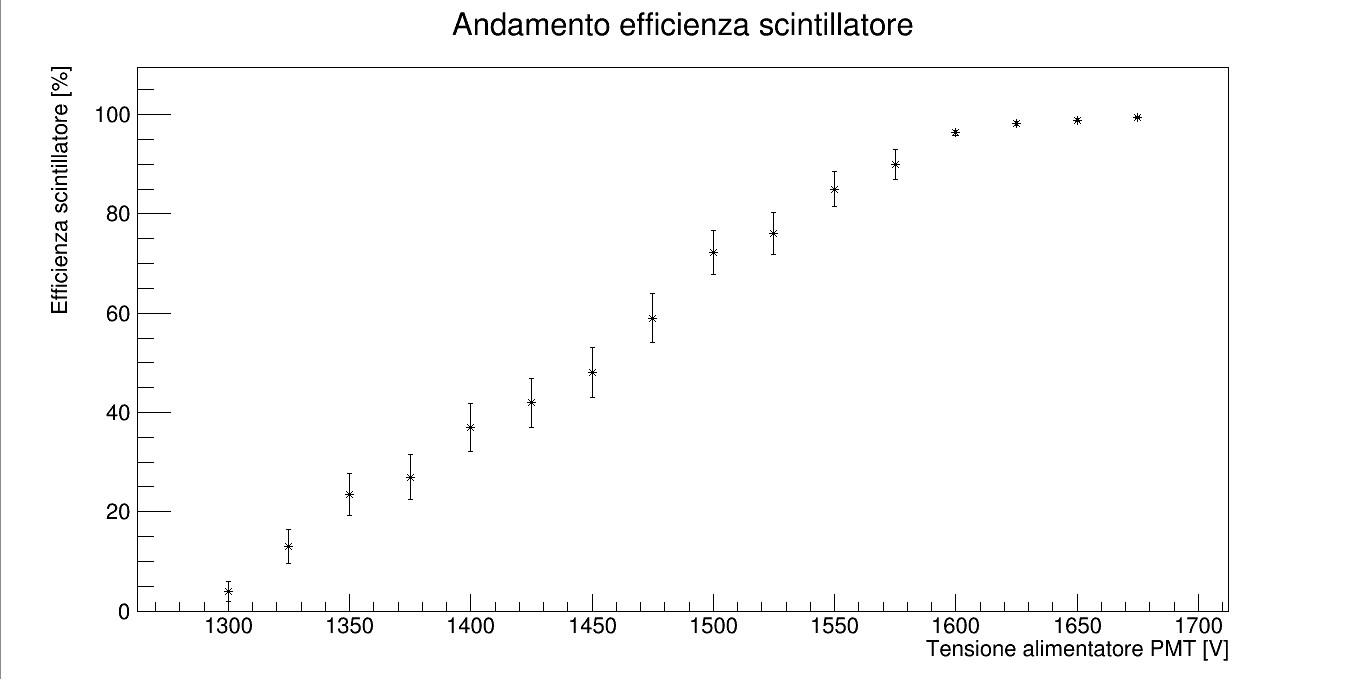
\includegraphics[width=\linewidth]{efficienza scintillatore.jpg} 
    \caption{Andamento dell'efficienza}
    \label{figura1}
\end{figure}
\begin{table}[h!]
  \begin{center}
   \begin{tabular}{|c|c|c|c|}
      V$_{\eta_{2}}$[V]&N$_{D}$&N$_{T}$&$\eta_{2}$[$\%$]\\
      1300&101&4&3.96$\pm$1.94\\
      1325&100&13&13.00$\pm$3.36\\
      1350&102&24&23.53$\pm$4.20\\
      1375&100&27&27.00$\pm$4.44\\
      1400&100&37&37$\pm$4.83\\
      1425&100&42&42.00$\pm$4.94\\
      1450&100&48&48.00$\pm$5.00\\
      1475&100&59&59.00$\pm$4.92\\
      1500&101&73&72.28$\pm$4.45\\
      1525&100&76&76.00$\pm$4.27\\
      1550&100&85&85.00$\pm$3.57\\
      1575&100&90&90.00$\pm$3.00\\
      1600&1200&1156&96.33$\pm$0.54\\
      1625&1200&1178&98.17$\pm$0.39\\
      1650&1200&1186&98.83$\pm$0.31\\
      1675&1200&1193&99.42$\pm$0.22\\
      \end{tabular}
  \caption{Tabella associata al grafico}
  \end{center}
\end{table}
\end{document}